\documentclass[11pt]{article}
% Packages
\usepackage[utf8]{inputenc}
\usepackage[T1]{fontenc}
\usepackage[margin=1in]{geometry}
\usepackage{amsmath, amsthm, amsfonts, amssymb}
\usepackage{mathrsfs}           % \mathscr font.
\usepackage{setspace}
\usepackage[colorlinks=true,linkcolor=blue,citecolor=blue,urlcolor=blue,breaklinks]{hyperref}
\usepackage{graphicx}
\usepackage{booktabs}
\usepackage{xcolor}
\usepackage[style = authoryear, autocite=inline, doi=false,isbn=false,url=false]{biblatex}
\usepackage[sc]{titlesec} % make section headings \sffamily

% Header styling
% make headers \sffamily
\newpagestyle{main}[\sffamily]{
    \sethead{\thepage}{}{\sectiontitle}
    }
\pagestyle{main}
\usepackage{titling}
% make titling elements \sffamily
\pretitle{\begin{center}\sc \LARGE}
\preauthor{\begin{center}
            \large\sffamily \lineskip 0.5em%
            \begin{tabular}[t]{c}}
\predate{\begin{center}\sffamily\large}
\usepackage{abstract}
% make abstract title \sffamily
\renewcommand\abstractnamefont{\sffamily}
\titleformat{\section}[block]{\filcenter \Large \sc}{\thesection}{1em}{}
\usepackage{caption}
\captionsetup{font=sf, labelfont = bf}

% Define symbols and maths shortcuts
\DeclareRobustCommand{\bbone}{\text{\usefont{U}{bbold}{m}{n}1}}
\DeclareMathOperator{\EX}{\mathbb{E}} % expected value
\DeclareMathOperator{\V}{\mathbb{V}}
\DeclareMathOperator{\Prob}{\mathbb{P}}
\newcommand*{\trans}{^{\mathsf{T}}} %matrix transpose

\usepackage[long, nodayofweek]{datetime}
\usepackage[style = authoryear]{biblatex}

\addbibresource{../../literature/leapfrogging.bib}
\AtEveryBibitem{\clearfield{month}}
\newtheorem{assumption}{Assumption}
\usepackage{tikz}

\title{Party Competition between Regional Parties: Diverging from the Median}
\author{Tobias Nowacki\thanks{Stanford University, Calif., USA. \texttt{tnowacki@stanford.edu}. With thanks to David Laitin and Apoorva Lal. This proposal is for a joint project with Apoorva Lal in mind.}}

% Begin Document
\begin{document}

\maketitle

\onehalfspacing

\section{Introduction}

Blurb about what we want to do with this paper.
Another blurb about what this research proposal does.
Why is this important?

\section{Literature and Motivation}

The idea of ethnic outbidding suggests that cross-ethnic or centrist coalitions cannot hold because its constituent ethnic parties are vulnerable to more extreme challengers; this results in a spiral of more and more extreme policy positions \parencite{Horowitz2000, Rabushka1972, Chandra2005}. Horowitz's contribution in particular sparked a large literature on ethnic politics; the term `ethnic outbidding' is widely used and referenced in relation to ethnicity-based parties. The role of elections in spurring ethnic conflict has also been considered (e.g., Cederman et al., 2012); however, this literature takes an \textit{ex post} perspective, analysing the likelihood of conflict after an election has taken place. Instead, the idea of ethnic outbidding suggests that there is something inherent about the \textit{ex ante} competition that leads to increasingly polarised positions and, at worst, conflict and the breakdown of the polity.

Empirically, the phenomenon of increasingly more extreme ethnic parties has been widely observed, both in established democratic politics, such as Northern Ireland / UK (references here) or Catalonia / Spain, as well as in developing countries (e.g., Sri Lanka, see DeVolta 2005; Moldova, see Kaufman 1996). (Include some more about Catalonia?)

Yet, the mechanism that leads to increasingly polarised parties has not resulted in a large formal-theoretical literature, for some reason. If we think of ethnicity as a continuous `policy dimension' with voters distributed across it, the classic Downsian model would predict convergence and a moderate stance. Furthermore, the threat from challengers implicitly assumes some form of entry mechanism that is not specified any clearer. Some attempts at a formalisation of the mechanism impose additional assumptions: in \textcite{Chandra2005}, for example, the depiction of Horowitz's theory requires that preferences are distributed fully dichotomously, doing away with a continuous distribution of voters.

The model developed in this research proposal seeks to connect to this literature by offering a novel mechanism through which we can explain ethnic parties settling in a policy position that is more extreme than the median. Although the motivation primarily comes from regional parties in Europe (e.g., Catalonia), the underlying model can be applied to other policy areas, too. The crucial assumption here is that the national distribution of preferences is centred around one extreme of the policy dimension, whereas the regional one is distributed evenly or in a polarised fashion across both.

Another key question is whether the empirically observed process of polarisation is driven by changes in voters' preferences, or induced by party elites (and parties' changing policy positions). This research proposal seeks to explain ethnic polarisation as an outcome of the latter (for party-driven `ethnic outbidding' in Catalonia, see \textcite{Barrio2017}). That said, elite-driven polarisation may later induce a shift in voters' preferences, too \parencite[p. 291]{Horowitz2000}, which further contributes to the destabilisation of the polity.

In summary, the idea for a contribution here is to offer a theory of multi-level elections, and how differences in the preference distribution between regional and national electorates can lead to divergence from the median voter position if multiple regional parties compete with each other. This can be applied to ethnicity or regional autonomy as examples of policy dimensions with strongly divergent preference distributions in the nation and the region; the regional competition may lead to parties advocating more extreme positions that may, in turn, threaten the unity of the polity and/or the democratic process.

\section{Theoretical framework: baseline}

The general framework of the model is as follows: let there be two separate elections - one at the national level, and one at the regional level, with separate electorates (or we can assume that the regional electorate is a subset of the national one). There is a continuuous, unidimensional policy space $P \in [0, 1]$. Our main policy dimension of interest is ethnicity, or regional autonomy, but this could be substituted for any other policy dimension that exhibits the kinds of differences described below.\footnote{Ethnicity here would not be dichotomous, but a continuous dimension, e.g., voters can feel half-Spanish, half-Catalan. Perhaps thinking about it in a 'regional autonomy' way (secession all the way to centralised state) is a better way.} Let the dimension range from 0 to 1. The distribution of preferences between the two electorates differs: the national electorate is tightly clustered around one extreme (the unionist one), such that the median voter $\tilde{v}_N = 0.9$, whereas the regional electorate is either uniform or polarised around both extremes, and $\tilde{v}_R = 0.5$. For now, assume that the regional electorate is distributed uniformly with support $[0, 1]$.

For the purpose of the baseline model, let there be one national party, $N$, that competes in both the national and the regional election, and up to two regional parties, $R_1, R_2$, that only compete in the regional elections. Furthermore, I impose the following two assumptions:

\begin{assumption}
    The national party runs in both the national and the regional election, but cares about winning office in the national election; the regional parties only run in the regional election and care about winning in it.
\end{assumption}
\begin{assumption}
    The national party can only set one policy position, $p_N$, with which it has to run in both elections.
\end{assumption}

Assumption 1 can be rationalised as follows: the national party cares about the `bigger' office but in order to bolster its claim that it is a nation-wide party, it also has to run in all sub-national elections regardless of whether it anticipates to win or not. (This is not unlike the Spanish Partido Popular in Spain / Catalonia). Regional parties, on the other hand, by default only care about the regional election. Assumption 2 follows from a model of parties as uniform and centralised actors, which may be especially fitting for unionist parties that seek greater centralisation.

Finally, for the purpose of this baseline model, let all parties be office-seeking, that is, they want to maximise their vote share.

It follows from Assumption 1 that $N$ will determine its policy position ($p_N$) with respect to the national electorate; following the median voter theorem, it will always position itself at the national median, such that $p_N = \tilde{v}_N$. From this follows that $N$ will also compete in the regional elections with the same policy position, which, however, is far to the right of the \textit{regional} median. In the next subsections, I will show how regional parties react to this setting and how this may lead to two regional parties to the left of the median voter in equilibrium. This result may offer a first shot at a formal mechanism for elite-driven 'ethnic outbidding'.


\subsection{One regional party}

\begin{figure}[ht]
    \centering 
     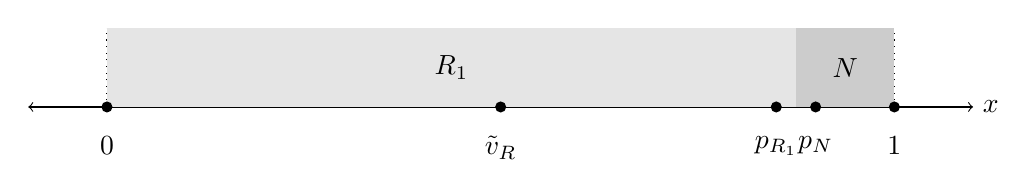
\begin{tikzpicture}
         % Axes
         \draw [<->] (-1,0) -- (11,0) node [right] {$x$};
         \draw [dotted] (0, 0) -- (0, 1);
         \draw [dotted] (10, 0) -- (10, 1);
         \draw [-] (0, 1) -- (10, 1);
         \fill [black!10] (0, 0) rectangle (8.75, 1);
         \draw (4.375, 0.5) node {$R_1$};
         \fill [black!20] (8.75, 0) rectangle (10, 1);
         \draw (9.375, 0.5) node {$N$};
         % Origin
         \node at (0,-.25) [below] {$0$};
         \node at (10, -.25) [below] {$1$};
         \node at (5, -.25) [below] {$\tilde{v}_R$};
         \node at (8.5, -.25) [below] {$p_{R_1}$};
         \node at (9, -.25) [below] {$p_{N}$};
         \coordinate (orig) at (0, 0);
         \coordinate (med)  at (5, 0);
         \coordinate (r1)   at (8.5, 0);
         \coordinate (N)    at (9, 0);
         \coordinate (end)  at (10, 0);
         \foreach \n in {orig, r1, med, N, end} \fill [black] (\n) circle (2pt);
     \end{tikzpicture}
     \caption{One national and one regional party; uniform distribution (regional electorate).} \label{fig:mod1}
 \end{figure}

 First, assume that there is only one regional party, $R_1$, that competes with $N$. 

 In equilibrium, it will position itself just to the left of $N$, and win the votes of everyone in the range from $[0, \frac{p_N + p_{R1}}{2}]$. $R_1$ has no incentive to move: moving further left would incur a vote loss towards $N$, and moving to the right of $N$ would leave them with a much smaller share of the distribution. Per assumption, $N$ cannot move its policy position. This is visualised in Figure \label{fig:mod1}. The resulting vote shares are $V_R = \frac{p_N + p_{R1}}{2}$ and $V_N = 1 - \frac{p_N + p_{R1}}{2}$.

As a consequence, the regional party positions itself close to the national party, and there is little issue competition on this dimension. Both are to the right of the regional median voter.\footnote{This is less problematic, because there is a reasonable argument that both the national and the regional party are close to the \textit{national} median voter. Whether that matters for evaluating the welfare outcome of this result for \textit{regional} elections is unclear.} It is likely that other divides (e.g., the classic left-right divide) are more salient in this scenario.

In practice, however, the regional party may position itself closer towards the median / the secessionist end, because of either inherent uncertainty or because of an intrinsic preference for a more autonomous policy. (see extensions to try and capture this. Another alternative is that they want to prevent any challengers from entering.) In either case, they will retain the majority of the vote share and thus capture office.\footnote{In the baseline model, the result suggests that they would be very close to $N$, purely because they'd rather win 90\% of the vote than `just' 60\%. That's not necessarily a plausible result, so the extensions may be crucial here.}

\subsection{Two regional parties}

\begin{figure}[ht]
    \centering 
     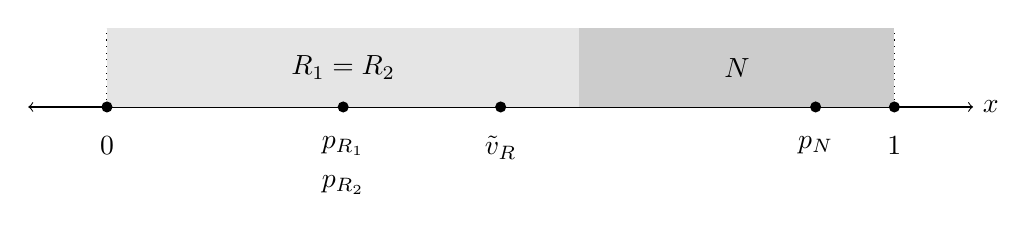
\begin{tikzpicture}
         % Axes
         \draw [<->] (-1,0) -- (11,0) node [right] {$x$};
         \draw [dotted] (0, 0) -- (0, 1);
         \draw [dotted] (10, 0) -- (10, 1);
         \draw [-] (0, 1) -- (10, 1);
         \fill [black!10] (0, 0) rectangle (6, 1);
         \draw (3, 0.5) node {$R_1 = R_2$};
         \fill [black!20] (6, 0) rectangle (10, 1);
         \draw (8, 0.5) node {$N$};
         % Origin
         \node at (0,-.25) [below] {$0$};
         \node at (5,-.25) [below] {$\tilde{v}_R$};
         \node at (10, -.25) [below] {$1$};
         \node at (3, -.25) [below] {$p_{R_1}$};
         \node at (3, -.75) [below] {$p_{R_2}$};
         \node at (9, -.25) [below] {$p_{N}$};
         \coordinate (orig) at (0, 0);
         \coordinate (med)  at (5, 0);
         \coordinate (r1)   at (3, 0);
         \coordinate (N)    at (9, 0);
         \coordinate (end)  at (10, 0);
         \foreach \n in {orig, r1, med, N, end} \fill [black] (\n) circle (2pt);
     \end{tikzpicture}
     \caption{One national and two regional parties; uniform distribution (regional electorate).} \label{fig:mod1}
 \end{figure}

Next, suppose that there are two regional parties, $R_1$ and $R_2$ that compete together with $N$. I keep the assumption of uniformly distributed voters for now, before discussing a more general case in the next subsection.

As before, $N$ keeps its policy position fixed at $p_N = \tilde{v}_N$. In equilibrium, both regional parties position themselves at $p_N / 3$, such that they split the voters in the range $[0, 2 p_N/3]$ between them. Their vote shares are thus $V_{R1} = V_{R2} = p_N / 3$, whereas $N$ receives $V_N = 1 - \frac{2}{3} p_N$. Here, neither regional party has an incentive to move. Moving leftwards would only decrease their vote share to below $p_N / 3$; moving rightwards they would only swap votes they would gain from $N$ with those lost to the other regional party. The best they could do by moving rightwards is to position themselves at $2/3 p_N$, which would see them gain the same vote share again; however, in this case, $R_2$ could move closer again in order to optimise their vote share (thus, $(p_N / 3, 2 p_N/3, p_N) $ cannot be an equilibrium). Finally, there is no incentive to move to $p_N$: the split vote share with $N$ would be smaller than the split vote share with $R_2$. Note that this imposes the constraint $p_N \geq 0.75$ for this to be an equilibrium.\footnote{The vote share that $R$ gets in equilibrium must be greater than the vote share it would get if it were to share its policy position with $N$ instead, that is, the inequality $v_R \geq V_N / 2$ or $\frac{1}{3} p_N \geq (1 - \frac{2}{3} p_N) / 2$ must hold. This simplifies to $p_N \geq 0.75$.}

This result shows how the competition between the two regional parties can drive them to take on more extreme policy positions that are to the left of the regional median voter, and certainly far to the left of the national median voter. This captures a possible mechanism for `ethnic outbidding': given the fixed policy position of the national party, and their proximity to unionist-minded voters, the two regional parties compete for the attachment of the regional ethnicity instead, thus forgoing the compromise position between the two (i.e., the median voter).

\subsection{Two regional parties, polarised distribution}

The result from the previous subsection can be stated more generally, as long as the underlying distribution of voters is symmetric around the median voter, and the density is weakly increasing on either side of the median voter.\footnote{With `humps' in the distribution, the equilibrium may not work, as parties may take up more than 1/3 of the share if it's tightly clustered together} $\rightarrow$ conditions for symmetric polarisation!

Let $f(x)$ denote the pdf of voters with support over the policy dimension, $x \in [0, 1]$; let $F(x)$ denote the cdf, and $F^{-1}(x)$ the inverse of the cdf or the quantile function.

The previous equilibrium can then be restated in terms of parties' vote shares:

\begin{align*}
    p_{R1} = p_{R2} & = F^{-1}\Big(\frac{F(N)}{3}\Big) \\
    p_N & = \tilde{v}_N
\end{align*}

and the corresponding vote shares are:

\begin{align*}
    V_{R1} = V_{R2} & = \frac{1}{2} \int_{0}^{F^{-1}(\frac{2 F(N)}{3})} f(x) dx = \frac{1}{3} \int_{0}^{p_N} f(x) dx \\
    V_N & = 1 - \frac{2}{3} \int_{0}^{p_N} f(x) dx = \int_{\frac{p_N + p_R}{2}}^{1} f(x) dx
\end{align*}

(express this in terms of the cdf...)

As the distribution becomes more polarised, $p_R$ will be further removed from the regional median voter (why? -- discuss intuition).

One way to model a symmetric polarised distribution is the beta distribution. Figure X plots the distribution of voters, parties policy points in equilibrium, and their share of voters, for different parameters of the beta distribution. (This confirms the previous point.)

% In the more general case (weaker assumption: symmetric distribution), the position will be such that they locate their policy position at the first tercile of the voter mass with support $[0, p_N]$, such that:

% \begin{equation*}
%     F^{-1}(R_1, R_2) = F^{-1}\Big(\frac{F(N)}{3}\Big) 
% \end{equation*}

% and the resulting vote share for either $R_1, R_2$ is:

% \begin{equation*}
%     V_{R1} = V_{R2} = \frac{1}{2} \int_{0}^{F^{-1}(\frac{2 F(N)}{3})} f(x) dx 
% \end{equation*}


Main result: the more polarised the distribution becomes, the bigger is the deviation from the median.

\subsection{Results and Comparative Statics}

\begin{itemize}
    \item When polarisation increases, parties will take more extreme positions
    \item The more accommodating the national party is, the more extreme will the positions of the regional parties be.
\end{itemize}

\begin{figure}
    \centering
    \includegraphics{../../output/polarisation.pdf}
    \caption{Equilibrium positions under different parameter values for Beta distribution.}
    \label{fig:betadist}
\end{figure}

\section{Extensions and challenges}

\subsection{Model extensions}

\textsc{Policy-oriented parties.}

\textsc{Uncertainty.}

\textsc{Electoral system.}

\textsc{Dynamics.}

\subsection{Empirical extension \& Application}



\section{Conclusion}


\renewcommand*{\mkbibnamefamily}[1]{\textsc{\textbf{#1}}}
\renewcommand*{\mkbibnamegiven}[1]{\textsc{#1}}
\printbibliography

\end{document}
